\subsection*{Partie A}

	\medskip

	\begin{enumerate}
		\item \begin{enumerate}
			\item On considère l'expérience aléatoire "la joueuse effectue un lancer franc". C'est une épreuve de Bernoulli dont le succès est l'événement "la joueuse réussi son lancer". La probabilité du succès est $p=\np{0,6}$.

			On répète cette expérience $n=5$ fois de manière identique et indépendante donc la variable aléatoire qui compte le nombre de succès suit la loi binomiale de paramètres $p=\np{0,6}$ et $n=5$.

			\item $P(X \geqslant 4)=P(X=4) + P(X=5)$.

			La calculatrice donne $P(X \geqslant 4) \approx \np{0,34}$. Cela signifie que pour environ 34\,\% des séries de 5 lancers francs de cette joueuse à l'entraînement, elle réussit au moins 4 des 5 lancers.
		\end{enumerate}

		\item \begin{enumerate}
			\item $\ds \begin{aligned}[t] P(Y \geqslant 1) &=1 - P(Y < 1) \\
				& =1 - P(Y=0)\quad \text{car $Y$ prend des valeurs entières entre 0 et $n$.}\\
				& = 1 - \binom{n}{0} \times \np{0,6}^0 \times \np{0,4}^n\\
				& =1 - \np{0,4}^n
			\end{aligned}$
			On a donc bien :\quad $P(Y \geqslant 1)  =1 - \np{0,4}^n$.

			\item Ici, on cherche $n$ tel que $P(Y \geqslant 1) \geqslant \np{0,9999}$.

			$\begin{aligned}[t] P(Y \geqslant 1) \geqslant \np{0,9999} &\iff 1- \np{0,4}^n \geqslant \np{0,9999}\\
			& \iff -\np{0,4}^n \leqslant -\np{0,0001}\\
			& \iff \np{0,4}^n \leqslant \np{0,0001}\quad \text{ car } -1 < 0\\
			& \iff n \ln\left( \np{0,4} \right) \leqslant \ln \left( \np{0,0001} \right)\\
			& \iff n \geqslant \frac{\ln \left( \np{0,0001} \right)}{\ln\left( \np{0,4} \right)} \quad \text{ car } \ln(0,4) < 0
			\end{aligned}$

			Or \quad $\dfrac{\ln \left( \np{0,0001} \right)}{\ln\left( \np{0,4} \right)} \approx \np{10,052}$.

			À partir de 11 lancers, la probabilité d'en réussir au moins un est supérieure à \np{0,9999}.

			\item Voici le script Python complété :
\begin{lstlisting}[style=python,xleftmargin=0.3\linewidth,xrightmargin=0.3\linewidth,numbers=none]
def basket():
	p = 0.6
	n = 1
	while p < 0.9999 :
		n = n + 1
		p = 1 - 0.4**n
	return n
\end{lstlisting}
		\end{enumerate}
	\end{enumerate}

	\subsection*{Partie B}

	\begin{enumerate}
		\item On représente la situation à l'aide d'un arbre de probabilité
		\begin{center}
			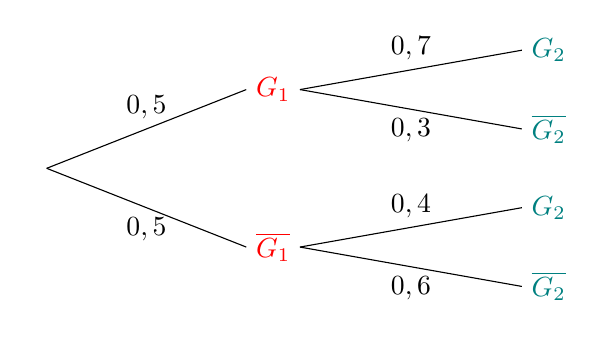
\begin{tikzpicture}
				[level 1/.style={level distance=3cm, sibling distance=2cm},
				level 2/.style={level distance=3.5cm,sibling distance=1cm},
				edge from parent path={(\tikzparentnode.east) -- (\tikzchildnode.west)}]
				\node {} [grow'=right]
				child {node {\textcolor{red}{$G_1$}}
					child {node {\textcolor{teal}{$G_2$}}
						edge from parent node[above] {$\np{0,7}$}
					}
					child {node {\textcolor{teal}{$\overline{G_2}$}}
						edge from parent node[below] {$\np{0,3}$}
					}
					edge from parent node[above] {$\np{0,5}$}
				}
				child {node {\textcolor{red}{$\overline{G_1}$}}
					child {node {\textcolor{teal}{$G_2$}}
						edge from parent node[above] {$\np{0,4}$}
					}
					child {node {\textcolor{teal}{$\overline{G_2}$}}
						edge from parent node[below] {$\np{0,6}$}
					}
					edge from parent node[below] {$\np{0,5}$}
				} ;
			\end{tikzpicture}
		\end{center}
		$G_1$ et $\overline{G_1}$ forment une partition de l'univers donc d'après la formule des probabilités totales, on a

		$\begin{aligned}[t] P\big( G_2 \big) &= P \big( G_1 \cap G_2 \big) + P \big( \overline{G_1} \cap G_2 \big)\\
		& = \np{0,5} \times \np{0,7} + \np{0,5} \times \np{0,4}\\
		& = \np{0,55}
		\end{aligned}$

		\item \begin{enumerate}
			\item \textbf{Initialisation.} Pour $n=1$, on a $p_1=\np{0,5}$ et $p_2=\np{0,55}$.

			On vérifie que $p_1 \leqslant p_2$ donc la propriété est vraie au rang 1.

			\textbf{Hérédité.} Soit $n$ un entier naturel non nul ($n\geqslant 1$), on suppose que l'inégalité est vraie pour cet entier $n$.
			Il faut démontrer que, pour cet entier $n \geqslant 1$, si $p_n \leqslant p_{n+1}$ alors $p_{n+1} \leqslant p_{n+2}$.

			D'après l'hypothèse de récurrence :\quad
			$\begin{aligned}[t] p_n \leqslant p_{n+1}
			& \Longrightarrow \np{0,3} p_n \leqslant \np{0,3} p_{n+1}\quad \text{ car }0,3 > 0\\
			& \Longrightarrow \np{0,3} p_n +\np{0,4} \leqslant \np{0,3} p_{n+1} + \np{0,4} \\
			& \Longrightarrow p_{n+1} \leqslant p_{n+2}
			\end{aligned}$

			Ainsi la propriété est héréditaire.

			\textbf{Conclusion.} La propriété est vraie au rang 1 et est héréditaire donc elle est vraie pour tout $n \geqslant 1$.

			On a donc pour tout $n \geqslant 1$,\quad $p_n \leqslant p_{n+1}$.

			Autrement dit, la suite $(p_n)$ est croissante.

			\item $p_n$ est la probabilité que le joueur réussisse son $n$-ième lancer franc, on a donc \quad $0 \leqslant p_n \leqslant 1$.

			La suite $(p_n)$ est bornée par 0 et 1, et donc elle est majorée par 1.

			\item D'après les deux questions précédentes, la suite $(p_n)$ est croissante et majorée par 1 : on en déduit qu'elle est convergente, vers une limite inférieure ou égale à 1.
		\end{enumerate}
		\item Le fait que la limite de $(p_n)$ quand $n$ tend vers $+\infty$ est $\dfrac47$ signifie qu'après un grand nombre de lancers francs, ce joueur va réussir en moyenne 4 lancers sur 7.
	\end{enumerate}

\needspace{10\baselineskip}
